\documentclass[12pt]{article}
\usepackage[english]{babel}
\usepackage[utf8x]{inputenc}
\usepackage[font=small,labelfont=bf]{caption}
\usepackage{amsmath}
\usepackage{graphicx}
\usepackage[colorinlistoftodos]{todonotes}
\usepackage{tabularx} % in the preamble

\begin{document}
	
	\begin{titlepage}
		
		\newcommand{\HRule}{\rule{\linewidth}{0.5mm}} % Defines a new command for the horizontal lines, change thickness here
		
		\center % Center everything on the page
		
		%----------------------------------------------------------------------------------------
		%	HEADING SECTIONS
		%----------------------------------------------------------------------------------------
		
		\textsc{\LARGE Central Washington University}\\[1.5cm] % Name of your university/college
		\textsc{\Large CS 471 OPTIMIZATION}\\[0.5cm] % Major heading such as course name
		\textsc{\large Spring 2019}\\[0.5cm] % Minor heading such as course title
		
		%----------------------------------------------------------------------------------------
		%	TITLE SECTION
		%----------------------------------------------------------------------------------------
		
		\HRule \\[0.4cm]
		{ \huge \bfseries Project 3 Report}\\[0.4cm] % Title of your document
		\HRule \\[1.5cm]
		
		%----------------------------------------------------------------------------------------
		%	AUTHOR SECTION
		%----------------------------------------------------------------------------------------
		
		\begin{minipage}{0.4\textwidth}
			\begin{flushleft} \large
				\emph{Author:}\\
				Hermann \textsc{Yepdjio} % Your name
			\end{flushleft}
		\end{minipage}
		~
		\begin{minipage}{0.4\textwidth}
			\begin{flushright} \large
				\emph{Supervisor:} \\
				Dr. Donald \textsc{Davendra} % Supervisor's Name
			\end{flushright}
		\end{minipage}\\[1cm]
		
		% If you don't want a supervisor, uncomment the two lines below and remove the section above
		%\Large \emph{Author:}\\
		%John \textsc{Smith}\\[3cm] % Your name
		
		%----------------------------------------------------------------------------------------
		%	DATE SECTION
		%----------------------------------------------------------------------------------------
		
		{\large \today}\\ % Date, change the \today to a set date if you want to be precise
		
		%----------------------------------------------------------------------------------------
		%	LOGO SECTION
		%----------------------------------------------------------------------------------------
		
		\includegraphics[width=12cm]{CWU-Logo.png}\\[.5cm] % Include a department/university logo - this will require the graphicx package
		
		%----------------------------------------------------------------------------------------
		
		\vfill % Fill the rest of the page with whitespace
		
	\end{titlepage}
	\newpage
	\tableofcontents
	\newpage
	
	
	
	\section{Introduction}
	For project 3, we were asked to optimize 18 standard benchmark functions namely Schwefel, De Jong 1, Rosenbrock's Saddle, Rastrigin, Griewangk, Sine Envelope Sine Wave, Stretch V Sine Wave, Ackley One, Ackley Two, Egg Holder, Rana, Pathological, Michalewicz, Master's Cosine Wave, Quartic, Levy, Step and Alpine. For this purpose, we've been given 2 optimization algorithms to be implemented then applied to those functions. Those algorithms are: Genetic Algorithm(GA) and Differential Evolution Algorithm (DE). After implementing them, we ran them on each of the 18 functions using randomly generated data. Statistics for each algorithm were computed and stored in a tabular format and they will be discussed then analyzed later on in this report. However, in order to observe how the fitness of each objective function varies across generations, we considered plotting the results for GA for one of the experiments.
	
		
	\section{Results}
	
		\subsection{Genetic Algorithm}
		
			\subsubsection{Values used for the parameters}
				The Genetic Algorithm was  run using  the following values:
				\begin{itemize}
					\item dimension: 30
					\item population size: 200
					\item number of generations: 100
					\item number of experiments: 50
					\item crossover rate: 0.8
					\item elitism rate: 0.2
					\item mutation range: 0.1
					\item mutation rate: 0.005
					\item mutation precision 5
				\end{itemize}
		
			\subsubsection{Statistics}
				% latex table generated in R 3.5.3 by xtable 1.8-4 package
				% Fri May  3 10:20:02 2019
				\begin{table}[hp!]
					\caption{Statistics for GA (50 experiments)}
					\centering
					\scalebox{.87}
					{
						\begin{tabular}{llllll}
							\hline
							& {\textbf{Average}} & {\textbf{Std\_Dev}} & {\textbf{Range}} & {\textbf{Median}} & {\textbf{Avg\_Time}} \\ 
							\hline
							{\textit{f1 Schwefel}} & 2058.26 & 438.72 & 1958.65 & 2067.10 & 60.68 \\ 
							{\textit{f2 De Jong 1}} & 3022.68 & 1433.06 & 4966.14 & 2830.41 & 41.52 \\ 
							{\textit{f3 Rosenbrock}} & 598618230.00 & 442278465.18 & 1922789500.00 & 499541500.00 & 59.54 \\ 
							{\textit{f4 Rastrigin}} & 28924.19 & 36251.34 & 150185.80 & 32706.70 & 68.70 \\ 
							{\textit{f5 Griewangk}} & 400.24 & 82.34 & 362.36 & 396.22 & 78.76 \\ 
							{\textit{f6 Sine Envelope}} & -35.95 & 1.08 & 4.79 & -35.92 & 118.08 \\ 
							{\textit{f7 Stretch V Sine}} & 10.15 & 0.00 & 0.00 & 10.15 & 117.88 \\ 
							{\textit{f8 Ackley One}} & 40.83 & 17.84 & 75.50 & 40.27 & 93.34 \\ 
							{\textit{f9 Ackley Two}} & 151.31 & 31.50 & 129.65 & 150.10 & 138.06 \\ 
							{\textit{f10 Egg Holder}} & -16331.62 & 1220.14 & 6204.60 & -16425.25 & 90.74 \\ 
							{\textit{f11 Rana}} & -10065.63 & 485.96 & 2003.84 & -10144.15 & 142.68 \\ 
							{\textit{f12 Pathological}} & -9.76 & 1.78 & 8.21 & -9.87 & 125.08 \\ 
							{\textit{f13 Michalewicz}} & -26.40 & 0.60 & 2.68 & -26.36 & 165.40 \\ 
							{\textit{f14 Masters’ Cosine}} & -15.67 & 0.00 & 0.00 & -15.67 & 104.80 \\ 
							{\textit{f15 Quartic}} & 94064256.00 & 81955817.35 & 454582300.00 & 73253600.00 & 106.86 \\ 
							{\textit{f16 Levy}} & 587.22 & 246.61 & 1052.16 & 577.08 & 117.78 \\ 
							{\textit{f17 Step}} & 3371.14 & 1422.10 & 6273.49 & 3317.80 & 43.36 \\ 
							{\textit{f18 Alpine}} & 29.94 & 6.52 & 32.80 & 29.17 & 53.40 \\ 
							\hline
						\end{tabular}
					}
				\end{table}
			
		\subsubsection{Statistics analysis}
		
			When comparing the statistics of the GA to those obtained for the iterative local search algorithm in the previous assignment, we can see that there is a huge improvement in the fitness of objective functions. For example, Table 1 above shows that in average, the best fitness for the Schwefel function was 2058.26 and for Rosenbrock's Saddle function was 5.98 * 10$^9$ while in the previous assignment we respectively got 8524.18 and 3.03 * 10$^{10}$. However, Table 1 also shows that some functions such as De Jong 1 produced worse results (3022.68) compared to 0.088 obtained with the iterative local search.
			\subsubsection{plots}
				\begin{minipage}{0.6\linewidth}
					\includegraphics[width=\linewidth]{1.png}
					\captionof{figure}{Schwefel (Experiment \#1)}
				\end{minipage}
				\hfill
				\begin{minipage}{0.6\linewidth}
					\includegraphics[width=\linewidth]{2.png}
					\captionof{figure}{De Jong 1 (Experiment \#1)}
				\end{minipage}
				\begin{minipage}{0.6\linewidth}
					\includegraphics[width=\linewidth]{3.png}
					\captionof{figure}{Rosenbrock (Experiment \#1)}
				\end{minipage}
				\hfill
				\begin{minipage}{0.6\linewidth}
					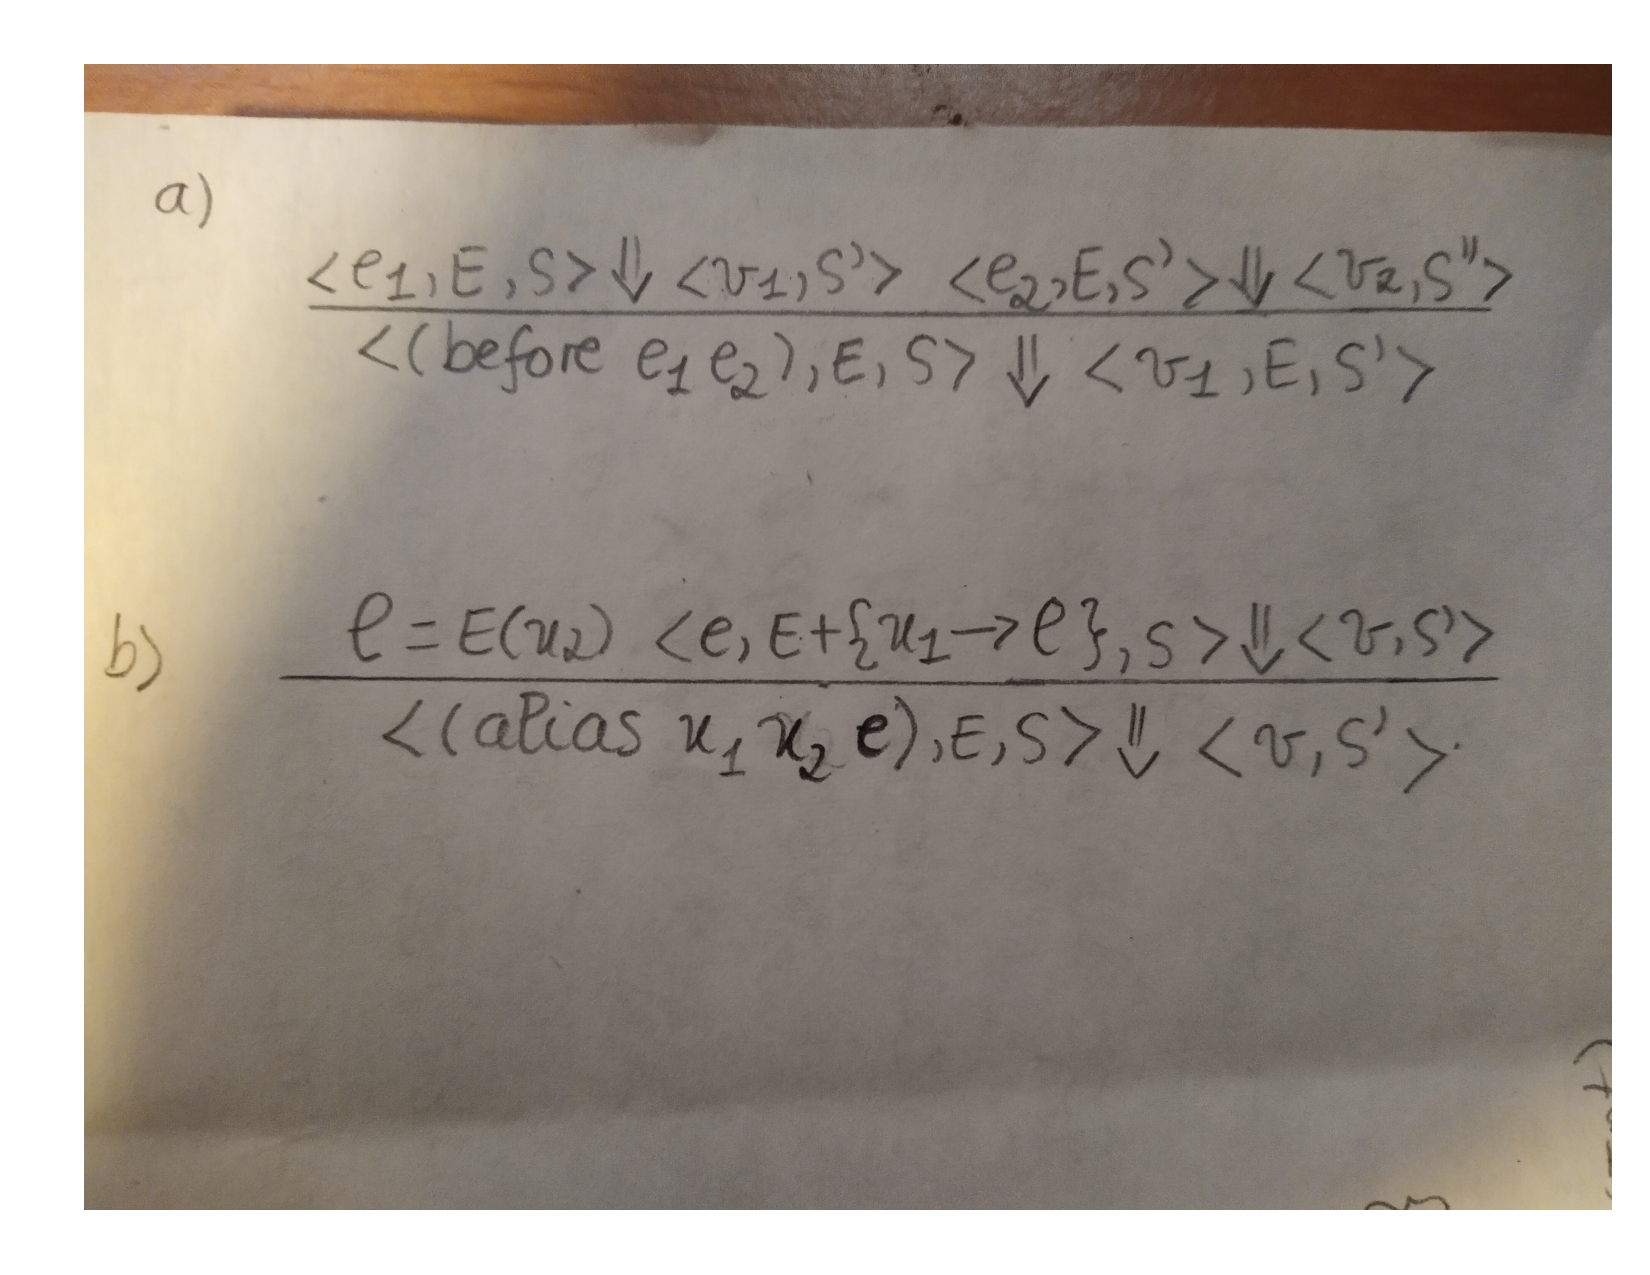
\includegraphics[width=\linewidth]{4.png}
					\captionof{figure}{Rastrigin (Experiment \#1)}
				\end{minipage}
				\begin{minipage}{0.6\linewidth}
					\includegraphics[width=\linewidth]{5.png}
					\captionof{figure}{Griewangk (Experiment \#1)}
				\end{minipage}
				\hfill
				\begin{minipage}{0.6\linewidth}
					\includegraphics[width=\linewidth]{6.png}
					\captionof{figure}{Sine Envelope (Experiment \#1)}
				\end{minipage}
				\begin{minipage}{0.6\linewidth}
					\includegraphics[width=\linewidth]{7.png}
					\captionof{figure}{Stretch V Sine (Experiment \#1)}
				\end{minipage}
				\hfill
				\begin{minipage}{0.6\linewidth}
					\includegraphics[width=\linewidth]{8.png}
					\captionof{figure}{Ackley One (Experiment \#1)}
				\end{minipage}
				\begin{minipage}{0.6\linewidth}
					\includegraphics[width=\linewidth]{9.png}
					\captionof{figure}{Ackley Two (Experiment \#1)}
				\end{minipage}
				\hfill
				\begin{minipage}{0.6\linewidth}
					\includegraphics[width=\linewidth]{10.png}
					\captionof{figure}{Egg Holder (Experiment \#1)}
				\end{minipage}
				\begin{minipage}{0.6\linewidth}
					\includegraphics[width=\linewidth]{11.png}
					\captionof{figure}{Rana (Experiment \#1)}
				\end{minipage}
				\hfill
				\begin{minipage}{0.6\linewidth}
					\includegraphics[width=\linewidth]{12.png}
					\captionof{figure}{Pathological (Experiment \#1)}
				\end{minipage}
				\begin{minipage}{0.6\linewidth}
					\includegraphics[width=\linewidth]{13.png}
					\captionof{figure}{Michalewicz (Experiment \#1)}
				\end{minipage}
				\hfill
				\begin{minipage}{0.6\linewidth}
					\includegraphics[width=\linewidth]{14.png}
					\captionof{figure}{Masters’ Cosine (Experiment \#1)}
				\end{minipage}
				\begin{minipage}{0.6\linewidth}
					\includegraphics[width=\linewidth]{15.png}
					\captionof{figure}{Quartic (Experiment \#1)}
				\end{minipage}
				\hfill
				\begin{minipage}{0.6\linewidth}
					\includegraphics[width=\linewidth]{16.png}
					\captionof{figure}{Levy (Experiment \#1)}
				\end{minipage}
				\begin{minipage}{0.6\linewidth}
					\includegraphics[width=\linewidth]{17.png}
					\captionof{figure}{Step (Experiment \#1)}
				\end{minipage}
				\hfill
				\begin{minipage}{0.6\linewidth}
					\includegraphics[width=\linewidth]{18.png}
					\captionof{figure}{Alpine (Experiment \#1)}
				\end{minipage}
			\subsubsection{Plots analysis}
				When looking at the figures above, we can see that the GA always improve the quality of the solutions as we go through generations except for 2 of the functions (Stretch V Sine (Figure 7) and Master's Cosine(Figure 14)). The reason to this improvement is that after each generation the algorithm gets rid of the bad solutions in both the original population and the new generated population and combines the rest to form the population for the next generation.
		
			\subsection{Differential Evolution Algorithm}
				\subsubsection{Values used for the parameters}
					The Differential Evolution Algorithm was  run using  the following values:
					\begin{itemize}
						\item dimension: 30
						\item population size: 200
						\item number of generations: 100
						\item number of experiments: 50
						\item crossover rate: 0.8
						\item F: 0.5
						\item $\lambda:$ 0.5
					\end{itemize}
				
					F and $\lambda$ were chosen by experimenting with different values for both and picking the ones that performed the best.
					
				\subsubsection{Statistics}
					% latex table generated in R 3.5.3 by xtable 1.8-4 package
					% Fri May  3 10:53:55 2019
					\begin{table}[hp!]
						\caption{Statistics for DE Strategy \#1 (50 Experiments)}
						\centering
						\scalebox{.87}
						{
							\begin{tabular}{llllll}
								\hline
								& {\textbf{Average}} & {\textbf{Std\_Dev}} & {\textbf{Range}} & {\textbf{Median}} & {\textbf{Avg\_Time}} \\ 
								\hline
								{\textit{f1 Schwefel}} & 9337.16 & 421.15 & 1763.05 & 9395.69 & 56.26 \\ 
								{\textit{f2 De Jong 1}} & 0.00 & 0.00 & 0.00 & 0.00 & 25.02 \\ 
								{\textit{f3 Rosenbrock}} & 23.5500000000 & 0.4700000000 & 2.1900000000 & 23.3600000000 & 43.68 \\ 
								{\textit{f4 Rastrigin}} & -89999.93 & 0.05 & 0.10 & -89999.90 & 44.74 \\ 
								{\textit{f5 Griewangk}} & 228045.76 & 18953.62 & 84384.00 & 227437.50 & 68.54 \\ 
								{\textit{f6 Sine Envelope}} & -26.68 & 1.05 & 4.40 & -26.55 & 107.76 \\ 
								{\textit{f7 Stretch V Sine}} & 10.15 & 0.00 & 0.00 & 10.15 & 105.06 \\ 
								{\textit{f8 Ackley One}} & -13.29 & 1.52 & 6.69 & -13.71 & 70.52 \\ 
								{\textit{f9 Ackley Two}} & -0.00 & 0.00 & 0.00 & -0.00 & 95.60 \\ 
								{\textit{f10 Egg Holder}} & -5174.36 & 599.35 & 2771.78 & -5165.21 & 100.52 \\ 
								{\textit{f11 Rana}} & -3404.17 & 586.65 & 2882.95 & -3325.24 & 172.66 \\ 
								{\textit{f12 Pathological}} & -7.89 & 1.21 & 5.24 & -7.66 & 114.50 \\ 
								{\textit{f13 Michalewicz}} & -8.29 & 0.87 & 5.31 & -8.22 & 162.26 \\ 
								{\textit{f14 Masters’ Cosine}} & -15.67 & 0.00 & 0.00 & -15.67 & 92.22 \\ 
								{\textit{f15 Quartic}} & 0.00 & 0.00 & 0.00 & 0.00 & 107.16 \\ 
								{\textit{f16 Levy}} & 1.76 & 0.34 & 1.58 & 1.74 & 103.88 \\ 
								{\textit{f17 Step}} & 7.25 & 0.00 & 0.00 & 7.25 & 25.68 \\ 
								{\textit{f18 Alpine}} & 0.00 & 0.00 & 0.00 & 0.00 & 26.00 \\ 
								\hline
							\end{tabular}
						}
					\end{table}
				
					% latex table generated in R 3.5.3 by xtable 1.8-4 package
					% Fri May  3 10:55:30 2019
					\begin{table}[bp!]
						\caption{Statistics for DE Strategy \#2 (50 Experiments)}
						\centering
						\scalebox{0.87}
						{
							\begin{tabular}{llllll}
								\hline
								& {\textbf{Average}} & {\textbf{Std\_Dev}} & {\textbf{Range}} & {\textbf{Median}} & {\textbf{Avg\_Time}} \\ 
								\hline
								{\textit{f1 Schwefel}} & 9508.19 & 341.21 & 1794.45 & 9489.93 & 56.20 \\ 
								{\textit{f2 De Jong 1}} & 0.00 & 0.00 & 0.00 & 0.00 & 24.76 \\ 
								{\textit{f3 Rosenbrock}} & 26.4300000000 & 0.3500000000 & 1.6000000000 & 26.4800000000 & 43.08 \\ 
								{\textit{f4 Rastrigin}} & -89999.94 & 0.05 & 0.10 & -89999.90 & 45.08 \\ 
								{\textit{f5 Griewangk}} & 693327.20 & 19787.04 & 82785.00 & 692252.00 & 51.66 \\ 
								{\textit{f6 Sine Envelope}} & -26.29 & 1.02 & 4.44 & -26.01 & 107.02 \\ 
								{\textit{f7 Stretch V Sine}} & 10.15 & 0.00 & 0.00 & 10.15 & 104.90 \\ 
								{\textit{f8 Ackley One}} & -7.99 & 0.55 & 2.55 & -7.90 & 71.00 \\ 
								{\textit{f9 Ackley Two}} & 0.01 & 0.01 & 0.02 & 0.01 & 103.52 \\ 
								{\textit{f10 Egg Holder}} & -4749.70 & 530.09 & 2288.92 & -4682.90 & 100.62 \\ 
								{\textit{f11 Rana}} & -3147.10 & 385.98 & 1576.27 & -3131.20 & 173.36 \\ 
								{\textit{f12 Pathological}} & -6.89 & 1.03 & 5.98 & -6.94 & 115.64 \\ 
								{\textit{f13 Michalewicz}} & -8.26 & 0.73 & 3.11 & -8.12 & 162.98 \\ 
								{\textit{f14 Masters’ Cosine}} & -15.67 & 0.00 & 0.00 & -15.67 & 93.16 \\ 
								{\textit{f15 Quartic}} & 0.00 & 0.00 & 0.00 & 0.00 & 105.40 \\ 
								{\textit{f16 Levy}} & 2.83 & 0.47 & 1.80 & 2.78 & 104.56 \\ 
								{\textit{f17 Step}} & 7.26 & 0.01 & 0.02 & 7.26 & 26.14 \\ 
								{\textit{f18 Alpine}} & 0.00 & 0.00 & 0.00 & 0.00 & 28.46 \\ 
								\hline
							\end{tabular}
						}
					\end{table}
					
					% latex table generated in R 3.5.3 by xtable 1.8-4 package
					% Fri May  3 10:56:12 2019
					\begin{table}[bp!]
						\caption{Statistics for DE Strategy \#3 (50 Experiments)}
						\centering
						\scalebox{0.87}
						{
							\begin{tabular}{llllll}
								\hline
								& {\textbf{Average}} & {\textbf{Std\_Dev}} & {\textbf{Range}} & {\textbf{Median}} & {\textbf{Avg\_Time}} \\ 
								\hline
								{\textit{f1 Schwefel}} & 9282.48 & 459.01 & 2341.60 & 9251.43 & 59.72 \\ 
								{\textit{f2 De Jong 1}} & 0.00 & 0.00 & 0.00 & 0.00 & 30.18 \\ 
								{\textit{f3 Rosenbrock}} & 24.2000000000 & 0.2200000000 & 1.1100000000 & 24.2700000000 & 48.26 \\ 
								{\textit{f4 Rastrigin}} & -90000.00 & 0.00 & 0.00 & -90000.00 & 47.48 \\ 
								{\textit{f5 Griewangk}} & 428530.68 & 98709.30 & 452746.00 & 417406.00 & 53.20 \\ 
								{\textit{f6 Sine Envelope}} & -27.28 & 1.01 & 4.46 & -26.83 & 104.42 \\ 
								{\textit{f7 Stretch V Sine}} & 10.15 & 0.00 & 0.00 & 10.15 & 110.26 \\ 
								{\textit{f8 Ackley One}} & -10.12 & 1.43 & 8.45 & -10.15 & 75.16 \\ 
								{\textit{f9 Ackley Two}} & 0.00 & 0.00 & 0.00 & 0.00 & 98.06 \\ 
								{\textit{f10 Egg Holder}} & -5297.41 & 800.25 & 3447.91 & -5161.18 & 100.54 \\ 
								{\textit{f11 Rana}} & -3570.28 & 664.87 & 3237.28 & -3385.80 & 168.12 \\ 
								{\textit{f12 Pathological}} & -6.41 & 1.41 & 5.54 & -6.13 & 117.36 \\ 
								{\textit{f13 Michalewicz}} & -7.60 & 0.63 & 3.28 & -7.55 & 165.04 \\ 
								{\textit{f14 Masters’ Cosine}} & -15.67 & 0.00 & 0.00 & -15.67 & 98.18 \\ 
								{\textit{f15 Quartic}} & 0.00 & 0.00 & 0.00 & 0.00 & 110.84 \\ 
								{\textit{f16 Levy}} & 4.02 & 0.93 & 3.60 & 4.03 & 108.90 \\ 
								{\textit{f17 Step}} & 7.25 & 0.00 & 0.00 & 7.25 & 31.18 \\ 
								{\textit{f18 Alpine}} & 0.00 & 0.00 & 0.00 & 0.00 & 31.30 \\ 
								\hline
							\end{tabular}
						}
					\end{table}
				
					% latex table generated in R 3.5.3 by xtable 1.8-4 package
					% Fri May  3 10:56:36 2019
					\begin{table}[bp!]
						\caption{Statistics for DE Strategy \#4 (50 Experiments)}
						\centering
						\scalebox{0.87}
						{
							\begin{tabular}{llllll}
								\hline
								& {\textbf{Average}} & {\textbf{Std\_Dev}} & {\textbf{Range}} & {\textbf{Median}} & {\textbf{Avg\_Time}} \\ 
								\hline
								{\textit{f1 Schwefel}} & 9208.07 & 421.61 & 1835.15 & 9252.95 & 61.36 \\ 
								{\textit{f2 De Jong 1}} & 0.00 & 0.00 & 0.00 & 0.00 & 28.00 \\ 
								{\textit{f3 Rosenbrock}} & 25.0400000000 & 0.2900000000 & 1.2800000000 & 25.1100000000 & 47.10 \\ 
								{\textit{f4 Rastrigin}} & -89999.92 & 0.04 & 0.20 & -89999.90 & 48.44 \\ 
								{\textit{f5 Griewangk}} & 737636.72 & 103294.12 & 572686.00 & 738333.50 & 57.60 \\ 
								{\textit{f6 Sine Envelope}} & -26.57 & 0.98 & 4.63 & -26.45 & 111.74 \\ 
								{\textit{f7 Stretch V Sine}} & 10.15 & 0.00 & 0.00 & 10.15 & 109.08 \\ 
								{\textit{f8 Ackley One}} & -11.43 & 1.27 & 6.76 & -11.65 & 75.52 \\ 
								{\textit{f9 Ackley Two}} & 0.00 & 0.00 & 0.00 & 0.00 & 106.48 \\ 
								{\textit{f10 Egg Holder}} & -4926.21 & 721.56 & 3107.01 & -4746.57 & 105.66 \\ 
								{\textit{f11 Rana}} & -3584.02 & 706.88 & 3482.63 & -3396.12 & 178.26 \\ 
								{\textit{f12 Pathological}} & -6.93 & 1.20 & 5.09 & -6.67 & 119.98 \\ 
								{\textit{f13 Michalewicz}} & -8.97 & 0.77 & 3.49 & -8.88 & 165.86 \\ 
								{\textit{f14 Masters’ Cosine}} & -15.67 & 0.00 & 0.00 & -15.67 & 97.76 \\ 
								{\textit{f15 Quartic}} & 0.00 & 0.00 & 0.00 & 0.00 & 110.64 \\ 
								{\textit{f16 Levy}} & 2.55 & 0.60 & 2.14 & 2.58 & 108.12 \\ 
								{\textit{f17 Step}} & 7.25 & 0.00 & 0.00 & 7.25 & 29.44 \\ 
								{\textit{f18 Alpine}} & 0.00 & 0.00 & 0.00 & 0.00 & 31.96 \\ 
								\hline
							\end{tabular}
						}
					\end{table}
				
					% latex table generated in R 3.5.3 by xtable 1.8-4 package
					% Fri May  3 10:57:09 2019
					\begin{table}[bp!]
						\caption{Statistics for DE Strategy \#5 (50 Experiments)}
						\centering
						\scalebox{0.87}
						{
							\begin{tabular}{llllll}
								\hline
								& {\textbf{Average}} & {\textbf{Std\_Dev}} & {\textbf{Range}} & {\textbf{Median}} & {\textbf{Avg\_Time}} \\ 
								\hline
								{\textit{f1 Schwefel}} & 9530.00 & 362.82 & 1669.31 & 9581.85 & 61.74 \\ 
								{\textit{f2 De Jong 1}} & 0.01 & 0.01 & 0.03 & 0.01 & 28.46 \\ 
								{\textit{f3 Rosenbrock}} & 26.7200000000 & 0.2300000000 & 1.0100000000 & 26.7100000000 & 47.48 \\ 
								{\textit{f4 Rastrigin}} & -89970.84 & 18.77 & 90.60 & -89973.25 & 50.24 \\ 
								{\textit{f5 Griewangk}} & 1047711.68 & 17696.39 & 90176.00 & 1045960.00 & 58.54 \\ 
								{\textit{f6 Sine Envelope}} & -26.14 & 0.88 & 4.26 & -25.93 & 111.22 \\ 
								{\textit{f7 Stretch V Sine}} & 10.15 & 0.00 & 0.00 & 10.15 & 109.58 \\ 
								{\textit{f8 Ackley One}} & -7.45 & 0.93 & 5.82 & -7.23 & 76.06 \\ 
								{\textit{f9 Ackley Two}} & 0.05 & 0.02 & 0.09 & 0.05 & 113.52 \\ 
								{\textit{f10 Egg Holder}} & -4772.57 & 600.81 & 2870.44 & -4753.55 & 105.70 \\ 
								{\textit{f11 Rana}} & -3161.64 & 377.44 & 1548.08 & -3150.41 & 179.26 \\ 
								{\textit{f12 Pathological}} & -6.35 & 1.08 & 4.53 & -6.15 & 119.72 \\ 
								{\textit{f13 Michalewicz}} & -8.62 & 0.72 & 3.61 & -8.58 & 168.94 \\ 
								{\textit{f14 Masters’ Cosine}} & -15.67 & 0.00 & 0.00 & -15.67 & 97.96 \\ 
								{\textit{f15 Quartic}} & 0.00 & 0.00 & 0.00 & 0.00 & 110.90 \\ 
								{\textit{f16 Levy}} & 3.78 & 0.63 & 2.44 & 3.84 & 109.38 \\ 
								{\textit{f17 Step}} & 7.30 & 0.02 & 0.07 & 7.30 & 29.74 \\ 
								{\textit{f18 Alpine}} & 0.01 & 0.00 & 0.03 & 0.01 & 35.12 \\ 
								\hline
							\end{tabular}
						}
					\end{table}
				
					% latex table generated in R 3.5.3 by xtable 1.8-4 package
					% Fri May  3 10:57:39 2019
					\begin{table}[bp!]
						\caption{Statistics for DE Strategy \#6 (50 Experiments)}
						\centering
						\scalebox{0.87}
						{
							\begin{tabular}{llllll}
								\hline
								& {\textbf{Average}} & {\textbf{Std\_Dev}} & {\textbf{Range}} & {\textbf{Median}} & {\textbf{Avg\_Time}} \\ 
								\hline
								{\textit{f1 Schwefel}} & 7417.08 & 650.60 & 2668.65 & 7345.21 & 91.80 \\ 
								{\textit{f2 De Jong 1}} & 0.00 & 0.00 & 0.00 & 0.00 & 60.60 \\ 
								{\textit{f3 Rosenbrock}} & 46.0500000000 & 71.190000000 & 359.7300000000 & 28.480000000 & 78.90 \\ 
								{\textit{f4 Rastrigin}} & -33146.56 & 6089.82 & 26704.20 & -32740.00 & 92.12 \\ 
								{\textit{f5 Griewangk}} & 7244545.80 & 513801.73 & 2221270.00 & 7253925.00 & 113.96 \\ 
								{\textit{f6 Sine Envelope}} & -24.13 & 0.79 & 4.32 & -24.06 & 143.76 \\ 
								{\textit{f7 Stretch V Sine}} & 10.15 & 0.00 & 0.00 & 10.15 & 139.56 \\ 
								{\textit{f8 Ackley One}} & -22.17 & 3.22 & 18.67 & -22.48 & 125.76 \\ 
								{\textit{f9 Ackley Two}} & 0.10 & 0.04 & 0.19 & 0.09 & 159.84 \\ 
								{\textit{f10 Egg Holder}} & -6994.73 & 862.74 & 3509.88 & -6877.15 & 139.18 \\ 
								{\textit{f11 Rana}} & -5464.64 & 791.08 & 3818.87 & -5340.44 & 205.32 \\ 
								{\textit{f12 Pathological}} & 5.80 & 1.03 & 4.65 & 5.94 & 151.74 \\ 
								{\textit{f13 Michalewicz}} & -12.96 & 0.83 & 4.63 & -12.95 & 191.36 \\ 
								{\textit{f14 Masters’ Cosine}} & -15.67 & 0.00 & 0.00 & -15.67 & 129.62 \\ 
								{\textit{f15 Quartic}} & 0.00 & 0.00 & 0.00 & 0.00 & 138.68 \\ 
								{\textit{f16 Levy}} & 1.65 & 0.12 & 0.51 & 1.63 & 144.02 \\ 
								{\textit{f17 Step}} & 7.28 & 0.01 & 0.03 & 7.28 & 61.76 \\ 
								{\textit{f18 Alpine}} & 3.02 & 6.11 & 29.18 & 0.32 & 81.64 \\ 
								\hline
							\end{tabular}
						}
					\end{table}
				
					% latex table generated in R 3.5.3 by xtable 1.8-4 package
					% Fri May  3 10:58:03 2019
					\begin{table}[bp!]
						\caption{Statistics for DE Strategy \#7 (50 Experiments)}
						\centering
						\scalebox{0.87}
						{
							\begin{tabular}{llllll}
								\hline
								& {\textbf{Average}} & {\textbf{Std\_Dev}} & {\textbf{Range}} & {\textbf{Median}} & {\textbf{Avg\_Time}} \\ 
								\hline
								{\textit{f1 Schwefel}} & 7387.95 & 361.91 & 1637.36 & 7393.95 & 93.36 \\ 
								{\textit{f2 De Jong 1}} & 4041.51 & 643.27 & 2909.20 & 4063.03 & 60.64 \\ 
								{\textit{f3 Rosenbrock}} & 26391402000.0 & 5649789703.8 & 28104100000.0 & 27218150000.0 & 83.20 \\ 
								{\textit{f4 Rastrigin}} & 109457.06 & 13790.10 & 61378.10 & 110926.00 & 93.10 \\ 
								{\textit{f5 Griewangk}} & 13854674.00 & 45412.80 & 217000.00 & 13856350.00 & 116.74 \\ 
								{\textit{f6 Sine Envelope}} & -22.87 & 0.66 & 3.28 & -22.80 & 145.46 \\ 
								{\textit{f7 Stretch V Sine}} & 10.15 & 0.00 & 0.00 & 10.15 & 142.76 \\ 
								{\textit{f8 Ackley One}} & 108.41 & 8.76 & 38.41 & 109.76 & 132.72 \\ 
								{\textit{f9 Ackley Two}} & 368.04 & 12.83 & 52.76 & 368.18 & 171.78 \\ 
								{\textit{f10 Egg Holder}} & -6916.23 & 435.76 & 1807.35 & -6864.38 & 140.40 \\ 
								{\textit{f11 Rana}} & -4949.63 & 408.11 & 1563.37 & -4916.11 & 210.12 \\ 
								{\textit{f12 Pathological}} & 6.67 & 0.77 & 3.87 & 6.87 & 153.96 \\ 
								{\textit{f13 Michalewicz}} & -9.61 & 0.45 & 1.88 & -9.60 & 202.64 \\ 
								{\textit{f14 Masters’ Cosine}} & -15.67 & 0.00 & 0.00 & -15.67 & 129.34 \\ 
								{\textit{f15 Quartic}} & 4113264400.00 & 931955135.31 & 3943420000.00 & 4234680000.00 & 140.78 \\ 
								{\textit{f16 Levy}} & 328.56 & 101.44 & 470.63 & 334.64 & 154.02 \\ 
								{\textit{f17 Step}} & 3505.00 & 465.34 & 2036.62 & 3527.32 & 61.82 \\ 
								{\textit{f18 Alpine}} & 225.62 & 19.52 & 97.24 & 227.74 & 85.52 \\ 
								\hline
							\end{tabular}
						}
					\end{table}
				
					% latex table generated in R 3.5.3 by xtable 1.8-4 package
					% Fri May  3 10:58:30 2019
					\begin{table}[bp!]
						\caption{Statistics for DE Strategy \#8 (50 Experiments)}
						\centering
						\scalebox{0.87}
						{
							\begin{tabular}{llllll}
								\hline
								& {\textbf{Average}} & {\textbf{Std\_Dev}} & {\textbf{Range}} & {\textbf{Median}} & {\textbf{Avg\_Time}} \\ 
								\hline
								{\textit{f1 Schwefel}} & 7512.93 & 435.09 & 2274.57 & 7525.68 & 131.70 \\ 
								{\textit{f2 De Jong 1}} & 0.18 & 0.09 & 0.55 & 0.16 & 97.96 \\ 
								{\textit{f3 Rosenbrock}} & 1273.00000000 & 1732.820000000 & 8855.34000000 & 564.970000000 & 116.32 \\ 
								{\textit{f4 Rastrigin}} & -25371.11 & 6804.06 & 30661.10 & -24912.85 & 129.42 \\ 
								{\textit{f5 Griewangk}} & 8477336.80 & 551493.58 & 2778570.00 & 8458935.00 & 152.28 \\ 
								{\textit{f6 Sine Envelope}} & -24.01 & 0.62 & 2.85 & -23.98 & 183.70 \\ 
								{\textit{f7 Stretch V Sine}} & 10.15 & 0.00 & 0.00 & 10.15 & 180.20 \\ 
								{\textit{f8 Ackley One}} & -10.93 & 5.91 & 28.52 & -11.15 & 168.90 \\ 
								{\textit{f9 Ackley Two}} & 3.41 & 1.67 & 7.99 & 3.21 & 202.68 \\ 
								{\textit{f10 Egg Holder}} & -7317.64 & 549.21 & 2600.15 & -7295.34 & 177.50 \\ 
								{\textit{f11 Rana}} & -5186.27 & 609.28 & 3033.31 & -5107.62 & 249.50 \\ 
								{\textit{f12 Pathological}} & 6.14 & 1.03 & 4.64 & 6.30 & 192.74 \\ 
								{\textit{f13 Michalewicz}} & -9.08 & 0.55 & 2.24 & -9.12 & 246.96 \\ 
								{\textit{f14 Masters’ Cosine}} & -15.67 & 0.00 & 0.00 & -15.67 & 169.08 \\ 
								{\textit{f15 Quartic}} & 6.74 & 7.86 & 37.36 & 3.92 & 175.82 \\ 
								{\textit{f16 Levy}} & 3720.77 & 1762.96 & 7403.88 & 3302.01 & 194.86 \\ 
								{\textit{f17 Step}} & 8.15 & 0.25 & 1.30 & 8.16 & 98.42 \\ 
								{\textit{f18 Alpine}} & 50.14 & 26.58 & 116.30 & 43.89 & 125.30 \\ 
								\hline
							\end{tabular}
						}
					\end{table}
					
					% latex table generated in R 3.5.3 by xtable 1.8-4 package
					% Fri May  3 10:58:52 2019
					\begin{table}[bp!]
						\caption{Statistics for DE Strategy \#9 (50 Experiments)}
						\centering
						\scalebox{0.87}
						{
							\begin{tabular}{llllll}
								\hline
								& {\textbf{Average}} & {\textbf{Std\_Dev}} & {\textbf{Range}} & {\textbf{Median}} & {\textbf{Avg\_Time}} \\ 
								\hline
								{\textit{f1 Schwefel}} & 7989.56 & 337.86 & 1490.71 & 8011.59 & 122.46 \\ 
								{\textit{f2 De Jong 1}} & 3823.80 & 760.63 & 3652.30 & 3728.08 & 85.90 \\ 
								{\textit{f3 Rosenbrock}} & 6369925800.00 & 2242623436.37 & 10721940000.00 & 6184335000.00 & 107.80 \\ 
								{\textit{f4 Rastrigin}} & 106067.78 & 24503.54 & 109420.50 & 105891.00 & 119.42 \\ 
								{\textit{f5 Griewangk}} & 12065738.00 & 199774.63 & 830400.00 & 12037500.00 & 143.86 \\ 
								{\textit{f6 Sine Envelope}} & -23.55 & 0.75 & 3.10 & -23.46 & 173.84 \\ 
								{\textit{f7 Stretch V Sine}} & 10.15 & 0.00 & 0.00 & 10.15 & 169.54 \\ 
								{\textit{f8 Ackley One}} & 110.69 & 12.14 & 54.00 & 110.08 & 158.98 \\ 
								{\textit{f9 Ackley Two}} & 331.37 & 21.38 & 104.24 & 331.48 & 197.82 \\ 
								{\textit{f10 Egg Holder}} & -6837.80 & 568.91 & 3016.48 & -6828.45 & 169.24 \\ 
								{\textit{f11 Rana}} & -4815.27 & 464.87 & 1819.31 & -4722.77 & 237.50 \\ 
								{\textit{f12 Pathological}} & 6.98 & 0.58 & 2.68 & 6.98 & 181.36 \\ 
								{\textit{f13 Michalewicz}} & -13.29 & 0.93 & 4.01 & -13.26 & 219.90 \\ 
								{\textit{f14 Masters’ Cosine}} & -15.67 & 0.00 & 0.00 & -15.67 & 159.96 \\ 
								{\textit{f15 Quartic}} & 842594780.00 & 256182497.88 & 1139491000.00 & 852945000.00 & 166.42 \\ 
								{\textit{f16 Levy}} & 74.71 & 19.62 & 97.40 & 72.59 & 176.64 \\ 
								{\textit{f17 Step}} & 3364.15 & 714.64 & 2906.21 & 3296.14 & 87.88 \\ 
								{\textit{f18 Alpine}} & 227.05 & 24.13 & 108.11 & 225.97 & 111.82 \\ 
								\hline
							\end{tabular}
						}
					\end{table}
				
					% latex table generated in R 3.5.3 by xtable 1.8-4 package
					% Fri May  3 10:59:22 2019
					\begin{table}[tp!]
						\caption{Statistics for DE Strategy \#10 (50 Experiments)}
						\centering
						\scalebox{0.87}
						{
							\begin{tabular}{llllll}
								\hline
								& {\textbf{Average}} & {\textbf{Std\_Dev}} & {\textbf{Range}} & {\textbf{Median}} & {\textbf{Avg\_Time}} \\ 
								\hline
								{\textit{f1 Schwefel}} & 7778.33 & 312.46 & 1510.50 & 7823.93 & 124.06 \\ 
								{\textit{f2 De Jong 1}} & 20574.54 & 2270.94 & 10077.50 & 20996.95 & 89.16 \\ 
								{\textit{f3 Rosenbrock}} & 31868718000.0 & 6328393234.5 & 26634200000.0 & 32337750000.0 & 113.80 \\ 
								{\textit{f4 Rastrigin}} & 571635.14 & 59008.57 & 257106.00 & 562412.50 & 121.18 \\ 
								{\textit{f5 Griewangk}} & 14610540.00 & 33319.18 & 185500.00 & 14612900.00 & 147.06 \\ 
								{\textit{f6 Sine Envelope}} & -22.71 & 0.62 & 2.51 & -22.55 & 176.16 \\ 
								{\textit{f7 Stretch V Sine}} & 10.15 & 0.00 & 0.00 & 10.15 & 174.00 \\ 
								{\textit{f8 Ackley One}} & 244.49 & 15.60 & 64.30 & 248.49 & 161.28 \\ 
								{\textit{f9 Ackley Two}} & 447.55 & 11.93 & 52.65 & 448.82 & 200.90 \\ 
								{\textit{f10 Egg Holder}} & -7139.87 & 491.67 & 2054.78 & -7050.31 & 171.42 \\ 
								{\textit{f11 Rana}} & -4999.77 & 390.24 & 1570.68 & -4949.47 & 240.28 \\ 
								{\textit{f12 Pathological}} & 6.31 & 0.69 & 2.52 & 6.48 & 185.36 \\ 
								{\textit{f13 Michalewicz}} & -10.09 & 0.45 & 1.81 & -10.08 & 230.62 \\ 
								{\textit{f14 Masters’ Cosine}} & -15.67 & 0.00 & 0.00 & -15.67 & 159.80 \\ 
								{\textit{f15 Quartic}} & 4434390000.00 & 1130333159.69 & 5527710000.00 & 4486845000.00 & 170.52 \\ 
								{\textit{f16 Levy}} & 3116.75 & 565.63 & 2600.20 & 3089.74 & 187.90 \\ 
								{\textit{f17 Step}} & 19514.28 & 2184.96 & 9502.10 & 19467.35 & 90.74 \\ 
								{\textit{f18 Alpine}} & 334.03 & 23.52 & 92.20 & 337.74 & 114.66 \\ 
								\hline
							\end{tabular}
						}
					\end{table}
				\newpage
				
				\subsubsection{Statistics Analysis}
				
					Tables 2-10 above show the statistics for strategies \#1 to \#10 of the DE  algorithm. The first observation that can be made when looking at those tables is that each of the 10 strategies produces better results for most functions than both the iterative local search implemented in project2 and the GA. Another observation is that each of the strategies works, better on some of the objective functions and worse on the others, than other strategies. For example, strategy \#4 (Table 5) has an average fitness of 0 for De Jong 1 and 9208.7 for  Schwefel while strategy \#10 (Table 11) has an average fitness of 3823.80 for De Jong 1 and 7989.56 for Schwefel. Similarly strategy \#3 (Table 4) has an average fitness of 24.2 for Rosenbrock and -90000 for  Rastrigin while strategy \#8 (Table 9) has an average fitness of 1273 for Rosenbrock  and -25371.11 for Rastrigin.
					
					Among all 10 strategies, 
					\begin{itemize}
						\item strategy \#1 produced the best results for Rosenbrock's Saddle (average fitness: 23.55), Griewangk (average fitness: 228045.76), Masters Cosine Wave(average fitness: -15.67), Step (average fitness: 43.36) and Alpine (average fitness: 507.1146) which are all also better than the GA results for the same functions respectively except for Griewangk where an average fitness of 400.23 was found with the GA. 
					
						\item Strategy \#2 produced the best results for De Jong 1 (average fitness: 0), Egg Holder (average fitness: Egg Holder), Rana (average fitness: -3147.1), Quartic (average fitness: 0) which are all better than the results obtained with GA for the same functions respectively.
					
						\item Strategy \#3 produced the best results for Sine Envelope Sine Wave (average fitness: -22.71), Stretch V Sine Wave (average fitness: 10.15), Ackley Two (average fitness: 0), Michalewicz (average fitness: -7.6) which are all also better than the results obtained with GA for the same functions respectively except for Stretch V Sine Wave where a similar value was obtained.
						
						\item Strategy \#5 produced the best results for Ackley One (average fitness: -7.45) which is also better than what was obtained with the GA for the same function.
						
						\item Strategy \#6 produced better results for pathological (average fitness: 5.8) and Levy (average fitness: 1.65) which are both also better that the results obtained with the GA for the same functions respectively.
						
						\item Strategy \#7 produced the best results for Schwefel (average fitness: 7387.95) which is worse than what was obtained with the GA for the same function (average fitness: 2058.25).
						
						\item Strategy \#8 produced the best results for Rastrigin (average fitness: -25371.11) which is also better than what was obtained with the GA for the same function.
					\end{itemize}
					
					
		\section{Conclusion}
			In conclusion, among all 10 strategies, strategies \#1 \#2 \#3 and \#6 appear to be the most efficient as each of them produced the best results for at least 2 of the 18 functions. 
			The DE is better in general than the iterative local search even though the latter sometimes produces better results for some of the functions such as for Griewangk and Sine Envelope Sine Wave.
			The DE is better in general than the GA even though the latter sometimes produces better results for some of the functions such as for Griewangk.
			The GA is better in general than the iterative local search even though the latter sometimes produces better results for some of the functions such as for De Jong 1, Sine Envelope Sine Wave, Egg holder, Rana, Michalewicz and Step.
			
\end{document}